%% img/FunctionComposition.tex
%% Copyright 2019 Andrea Berlingieri
%
% This work may be distributed and/or modified under the
% conditions of the LaTeX Project Public License, either version 1.3
% of this license or (at your option) any later version.
% The latest version of this license is in
%   http://www.latex-project.org/lppl.txt
% and version 1.3 or later is part of all distributions of LaTeX
% version 2005/12/01 or later.
%
% This work has the LPPL maintenance status `maintained'.
%
% The Current Maintainer of this work is Andrea Berlingieri.
%
% This work consists of all files listed in manifest.txt
\documentclass{standalone}

\usepackage{TikzStyle}
\usepackage{mystyle}

\newcommand{\gpoint}[2]{%
\filldraw [gray] (#1,#2) circle [radius=2pt]
}

\begin{document}
    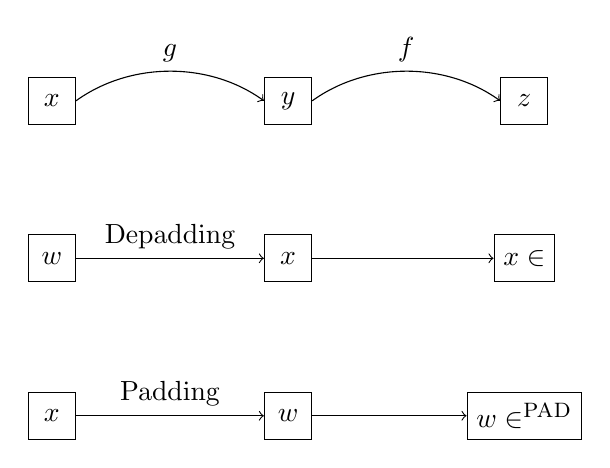
\begin{tikzpicture}
        \node[draw,minimum size=6mm] (x) at (0,0) {$x$};
        \node[draw,minimum size=6mm] (y) at (3,0) {$y$};
        \node[draw,minimum size=6mm] (z) at (6,0) {$z$};
        \draw[->] (x.east) .. controls (1,0.5) and (2,0.5) .. (y.west) node [pos=0.5,above] {$g$};
        \draw[->] (y.east) .. controls (4,0.5) and (5,0.5) .. (z.west) node [pos=0.5,above] {$f$};
        \node[draw,minimum size=6mm] (w1) at (0,-2) {$w$};
        \node[draw,minimum size=6mm] (x1) at (3,-2) {$x$};
        \node[draw,minimum size=6mm] (x1inL) at (6,-2) {$x \in \Lang$};
        \draw[->] (w1) -- (x1) node [pos=0.5,above] {Depadding};
        \draw[->] (x1) -- (x1inL);

        \node[draw,minimum size=6mm] (x2) at (0,-4) {$x$};
        \node[draw,minimum size=6mm] (w2) at (3,-4) {$w$};
        \node[draw,minimum size=6mm] (w2inLPad) at (6,-4) {$w \in \Lang^{\textsc{pad}}$};
        \draw[->] (x2) -- (w2) node [pos=0.5,above] {Padding};
        \draw[->] (w2) -- (w2inLPad);
    \end{tikzpicture}
\end{document}
